\documentclass[10pt,letter,oneside]{scrbook}
\usepackage[landscape]{geometry}
\usepackage{caption}
\usepackage{etoolbox}
\usepackage[final]{grffile}
\usepackage{graphicx}
\usepackage{fancyvrb}
\usepackage[T1]{fontenc}
\usepackage{fancyhdr}
\usepackage{listings}
\usepackage{lscape}
\usepackage{calc}
\graphicspath{{/home/mkg/Dropbox/images/}}
\pagestyle{headings}
\usepackage{lipsum}
\usepackage{url}
\usepackage[hidelinks=true,linktoc=all]{hyperref}
\urlstyle{same}
\usepackage[all]{hypcap}
\setlength{\parindent}{0em}
\setlength{\parskip}{1ex}
\begin{document}
	\frontmatter
	\onecolumn
	
	\title{Selected Photographs \\ Volume II}
	\author{Michael Gogins \\ \texttt{michael.gogins@gmail.com}}
	
	\maketitle
	
	\clearpage
	\noindent This book and all images therein are copyright 2020 by Michael Gogins, all rights reserved. The contents of this book are licensed under the terms of the Creative Commons \href{https://creativecommons.org/licenses/by-nc-nd/4.0/legalcode}{\textbf{Attribution-NonCommercial-NoDerivatives 4.0 International} } license. 
	
	In short, you may use, print, and copy this book or any of its contents for your own personal use, but you may not use this book or any of its contents as part of your own projects, or for commercial purposes.
	
	If you wish to use this book or any of its contents for your own projects, or for commercial purposes, for example to re-publish or to exhibit in a gallery, please contact me directly.
	
	\clearpage
	\begin{centering}
	This book is for Mick.
	\end{centering}
	
	\tableofcontents
	\listoffigures
	
	\mainmatter
	\lstset{language=c++,basicstyle=\ttfamily\scriptsize,commentstyle=\ttfamily\tiny,tabsize=2,breaklines,fontadjust=true,keepspaces=false,showstringspaces=false,moredelim=[is][\textbf]{\\emph\{}{\}}}
	
	\pagestyle{headings}
	\twocolumn
	\chapter{Introduction}
	
	This book contains my selection of pictures from a lifetime of taking photographs. I have never been a professional, but I was and am committed to the art of photography. I am a ``street photographer`` open to abstraction. I shoot what catches my eye and I prize beauty. When I take pictures of people, I often prefer they don't notice. My reason for doing photography is to see more clearly what God has created.
	
	These pictures were variously taken with 35 mm film cameras, a variety of digital cameras, and smartphones. They were taken in ny native state of Utah, other states including Washington, California, and New York, and countries around the world. I have tended to use the sharpest possible camera that is small enough to carry with me at all times. For some years now I have been using the Sony RX100 series. Increasingly, however, I am finding that my smartphone is a real camera.
	
	The images are all in natural color. They are all shot as far as possible without image manipulation; in a few cases, I have leveled horizons or removed spots. I shoot in JPEG rather than RAW. Selected metadata from the photographs is printed. If the photograph is a digital scan of a 35 mm slide, the creation date is the date of that scan. Captions are sporadic and cryptic, to say the least.
	
	All pictures are included in the full resolution with which they were taken. Thus, you can zoom into any image to see more detail. Pictures copied out of this book will also be in full resolution. As the file size of this book would otherwise become unmanageable thanks to the use of uncompressed images, it has been split into a number of volumes. Even so, the files are huge. However, they do enable the reader to zoom into the images in full detail or to extract them for printing at high resolution. I invite the reader to copy pictures out of this book for printing and viewing, but not for commercial use or re-publication. 
	
	If I take more pictures that I think are good enough to be in this book, I will add new volumes.
	
	\chapter{Photographs}
	
	
\clearpage
\onecolumn
\noindent 
\noindent
\begin{lstlisting}

Filename: SM-950U/20190411_114936.jpg

Date: 2019:04:11 11:49:36
GPS longitude: (175.0, 9.0, 31.8826)
GPS latitude: (37.0, 33.0, 50.9707)
Make: samsung
Model: SM-N950U
Focal length (35mm eq): 26
Exposure: 0.02
F stop: 1.7
ISO: 80
Width: 4032
Height: 1960
\end{lstlisting}
\clearpage

\begin{figure}
\includegraphics[width=\linewidth,height=\textheight,keepaspectratio,bb= 0 0 4032 1960]{/home/mkg/Dropbox/images/SM-950U/20190411_114936.jpg}
\captionlistentry[figure]{\url{\protect\detokenize{SM-950U/20190411_114936.jpg}}}
\end{figure}
    
\clearpage
\onecolumn
\noindent 
\noindent
\begin{lstlisting}

Filename: SM-950U/20190409_150209.jpg

Date: 2019:04:09 15:02:09
GPS longitude: (174.0, 19.0, 20.4895)
GPS latitude: (41.0, 12.0, 51.4366)
Make: samsung
Model: SM-N950U
Focal length (35mm eq): 26
Exposure: 0.00037537537537537537
F stop: 1.7
ISO: 50
Width: 4032
Height: 1960
\end{lstlisting}
\clearpage

\begin{figure}
\includegraphics[width=\linewidth,height=\textheight,keepaspectratio,bb= 0 0 4032 1960]{/home/mkg/Dropbox/images/SM-950U/20190409_150209.jpg}
\captionlistentry[figure]{\url{\protect\detokenize{SM-950U/20190409_150209.jpg}}}
\end{figure}
    
\clearpage
\onecolumn
\noindent 
\noindent
\begin{lstlisting}

Filename: SM-950U/20190407_154615.jpg

Date: 2019:04:07 15:46:15
GPS longitude: (172.0, 13.0, 43.5747)
GPS latitude: (42.0, 9.0, 39.0379)
Make: samsung
Model: SM-N950U
Focal length (35mm eq): 52
Exposure: 0.0017006802721088435
F stop: 2.4
ISO: 25
Width: 4032
Height: 1960
\end{lstlisting}
\clearpage

\begin{figure}
\includegraphics[width=\linewidth,height=\textheight,keepaspectratio,bb= 0 0 4032 1960]{/home/mkg/Dropbox/images/SM-950U/20190407_154615.jpg}
\captionlistentry[figure]{\url{\protect\detokenize{SM-950U/20190407_154615.jpg}}}
\end{figure}
    
\clearpage
\onecolumn
\noindent 
\noindent
\begin{lstlisting}

Filename: XT_1585/Camera/IMG_20170310_145854935.jpg

Date: 2017:03:10 14:58:55
Make: Motorola
Model: XT1585
Exposure: 0.00064
F stop: 2.0
ISO: 50
Width: 5344
Height: 3006
\end{lstlisting}
\clearpage

\begin{figure}
\includegraphics[width=\linewidth,height=\textheight,keepaspectratio,bb= 0 0 5344 3006]{/home/mkg/Dropbox/images/XT_1585/Camera/IMG_20170310_145854935.jpg}
\captionlistentry[figure]{\url{\protect\detokenize{XT_1585/Camera/IMG_20170310_145854935.jpg}}}
\end{figure}
    
\clearpage
\onecolumn
\noindent Scan of a slide, visual poet Karl Kempton.
\noindent
\begin{lstlisting}

Filename: renamed/c_2013-03-11_04-42-42.1.jpg

Make: Nikon
Model: Nikon SUPER COOLSCAN 5000 ED
Width: 5782
Height: 3946
\end{lstlisting}
\clearpage

\begin{figure}
\includegraphics[width=\linewidth,height=\textheight,keepaspectratio,bb= 0 0 4337 2960]{/home/mkg/Dropbox/images/renamed/c_2013-03-11_04-42-42.1.jpg}
\captionlistentry[figure]{\url{\protect\detokenize{renamed/c_2013-03-11_04-42-42.1.jpg}}}
\end{figure}
    
\clearpage
\onecolumn
\noindent Scan of a slide, Pacific shore near Karl Kempton's house, Avila Beach, California.
\noindent
\begin{lstlisting}

Filename: renamed/c_2013-03-11_04-42-41.1.jpg

Make: Nikon
Model: Nikon SUPER COOLSCAN 5000 ED
Width: 5782
Height: 3946
\end{lstlisting}
\clearpage

\begin{figure}
\includegraphics[width=\linewidth,height=\textheight,keepaspectratio,bb= 0 0 104 71]{/home/mkg/Dropbox/images/renamed/c_2013-03-11_04-42-41.1.jpg}
\captionlistentry[figure]{\url{\protect\detokenize{renamed/c_2013-03-11_04-42-41.1.jpg}}}
\end{figure}
    
\clearpage
\onecolumn
\noindent Scan of a slide, collectibles shop window, Venice Beach, California.
\noindent
\begin{lstlisting}

Filename: renamed/c_2013-03-11_04-42-39.1.jpg

Make: Nikon
Model: Nikon SUPER COOLSCAN 5000 ED
Width: 5782
Height: 3946
\end{lstlisting}
\clearpage

\begin{figure}
\includegraphics[width=\linewidth,height=\textheight,keepaspectratio,bb= 0 0 4337 2960]{/home/mkg/Dropbox/images/renamed/c_2013-03-11_04-42-39.1.jpg}
\captionlistentry[figure]{\url{\protect\detokenize{renamed/c_2013-03-11_04-42-39.1.jpg}}}
\end{figure}
    
\clearpage
\onecolumn
\noindent Scan of a slide, amusement park midway, The Pike, Long Beach, California, probably 1973 or 1974.
\noindent
\begin{lstlisting}

Filename: renamed/c_2013-03-11_04-42-38.1.jpg

Make: Nikon
Model: Nikon SUPER COOLSCAN 5000 ED
Width: 5782
Height: 3946
\end{lstlisting}
\clearpage

\begin{figure}
\includegraphics[width=\linewidth,height=\textheight,keepaspectratio,bb= 0 0 4337 2960]{/home/mkg/Dropbox/images/renamed/c_2013-03-11_04-42-38.1.jpg}
\captionlistentry[figure]{\url{\protect\detokenize{renamed/c_2013-03-11_04-42-38.1.jpg}}}
\end{figure}
    
\clearpage
\onecolumn
\noindent Scan of a slide, glass of ginger ale, Venice Beach, California, probably 1975.
\noindent
\begin{lstlisting}

Filename: renamed/c_2013-03-11_04-42-37.1.jpg

Make: Nikon
Model: Nikon SUPER COOLSCAN 5000 ED
Width: 5782
Height: 3946
\end{lstlisting}
\clearpage

\begin{figure}
\includegraphics[width=\linewidth,height=\textheight,keepaspectratio,bb= 0 0 104 71]{/home/mkg/Dropbox/images/renamed/c_2013-03-11_04-42-37.1.jpg}
\captionlistentry[figure]{\url{\protect\detokenize{renamed/c_2013-03-11_04-42-37.1.jpg}}}
\end{figure}
    
\clearpage
\onecolumn
\noindent Scan of a slide.
\noindent
\begin{lstlisting}

Filename: renamed/c_2013-03-11_04-42-35.1.jpg

Make: Nikon
Model: Nikon SUPER COOLSCAN 5000 ED
Width: 5782
Height: 3946
\end{lstlisting}
\clearpage

\begin{figure}
\includegraphics[width=\linewidth,height=\textheight,keepaspectratio,bb= 0 0 4337 2960]{/home/mkg/Dropbox/images/renamed/c_2013-03-11_04-42-35.1.jpg}
\captionlistentry[figure]{\url{\protect\detokenize{renamed/c_2013-03-11_04-42-35.1.jpg}}}
\end{figure}
    
\clearpage
\onecolumn
\noindent Scan of a slide, the merry-go-round in Griffith Park, Los Angeles, California, probably 1975 or 1976.
\noindent
\begin{lstlisting}

Filename: renamed/c_2013-03-11_04-42-31.1.jpg

Make: Nikon
Model: Nikon SUPER COOLSCAN 5000 ED
Width: 5782
Height: 3946
\end{lstlisting}
\clearpage

\begin{figure}
\includegraphics[width=\linewidth,height=\textheight,keepaspectratio,bb= 0 0 104 71]{/home/mkg/Dropbox/images/renamed/c_2013-03-11_04-42-31.1.jpg}
\captionlistentry[figure]{\url{\protect\detokenize{renamed/c_2013-03-11_04-42-31.1.jpg}}}
\end{figure}
    
\clearpage
\onecolumn
\noindent Scan of a slide, stream bed, Uinta Mountains, Utah, probably 1977 or 1978.
\noindent
\begin{lstlisting}

Filename: renamed/c_2013-03-11_04-42-30.1.jpg

Make: Nikon
Model: Nikon SUPER COOLSCAN 5000 ED
Width: 5782
Height: 3946
\end{lstlisting}
\clearpage

\begin{figure}
\includegraphics[width=\linewidth,height=\textheight,keepaspectratio,bb= 0 0 104 71]{/home/mkg/Dropbox/images/renamed/c_2013-03-11_04-42-30.1.jpg}
\captionlistentry[figure]{\url{\protect\detokenize{renamed/c_2013-03-11_04-42-30.1.jpg}}}
\end{figure}
    
\clearpage
\onecolumn
\noindent Scan of a slide, from the summit of Mount Whitney, Sierra Nevada Mountains, California, probably 1975.
\noindent
\begin{lstlisting}

Filename: renamed/c_2013-03-11_04-42-28.1.jpg

Make: Nikon
Model: Nikon SUPER COOLSCAN 5000 ED
Width: 5782
Height: 3946
\end{lstlisting}
\clearpage

\begin{figure}
\includegraphics[width=\linewidth,height=\textheight,keepaspectratio,bb= 0 0 104 71]{/home/mkg/Dropbox/images/renamed/c_2013-03-11_04-42-28.1.jpg}
\captionlistentry[figure]{\url{\protect\detokenize{renamed/c_2013-03-11_04-42-28.1.jpg}}}
\end{figure}
    
\clearpage
\onecolumn
\noindent Scan of a slide. The rounded summit at one o'clock high is Mount Whitney, Sierra Nevada Mountains, California, probably 1975.
\noindent
\begin{lstlisting}

Filename: renamed/c_2013-03-11_04-42-27.1.jpg

Make: Nikon
Model: Nikon SUPER COOLSCAN 5000 ED
Width: 5782
Height: 3946
\end{lstlisting}
\clearpage

\begin{figure}
\includegraphics[width=\linewidth,height=\textheight,keepaspectratio,bb= 0 0 104 71]{/home/mkg/Dropbox/images/renamed/c_2013-03-11_04-42-27.1.jpg}
\captionlistentry[figure]{\url{\protect\detokenize{renamed/c_2013-03-11_04-42-27.1.jpg}}}
\end{figure}
    
\clearpage
\onecolumn
\noindent Scan of a slide, near Alvarado Street, Los Angeles, California, mid to late 1970s.
\noindent
\begin{lstlisting}

Filename: renamed/c_2013-03-11_04-42-26.1.jpg

Make: Nikon
Model: Nikon SUPER COOLSCAN 5000 ED
Width: 3946
Height: 5782
\end{lstlisting}
\clearpage

\begin{figure}
\includegraphics[width=\linewidth,height=\textheight,keepaspectratio,bb= 0 0 2960 4337]{/home/mkg/Dropbox/images/renamed/c_2013-03-11_04-42-26.1.jpg}
\captionlistentry[figure]{\url{\protect\detokenize{renamed/c_2013-03-11_04-42-26.1.jpg}}}
\end{figure}
    
\clearpage
\onecolumn
\noindent Scan of a slide, doorway, Avila Beach, California. probably 1975 or 1976.
\noindent
\begin{lstlisting}

Filename: renamed/c_2013-03-11_04-42-24.1.jpg

Make: Nikon
Model: Nikon SUPER COOLSCAN 5000 ED
Width: 5750
Height: 3900
\end{lstlisting}
\clearpage

\begin{figure}
\includegraphics[width=\linewidth,height=\textheight,keepaspectratio,bb= 0 0 103 70]{/home/mkg/Dropbox/images/renamed/c_2013-03-11_04-42-24.1.jpg}
\captionlistentry[figure]{\url{\protect\detokenize{renamed/c_2013-03-11_04-42-24.1.jpg}}}
\end{figure}
    
\clearpage
\onecolumn
\noindent Scan of a slide, movie theater on Broadway, downtown Los Angeles, probably 1974 or 1975.
\noindent
\begin{lstlisting}

Filename: renamed/c_2013-03-11_04-42-23.1.jpg

Make: Nikon
Model: Nikon SUPER COOLSCAN 5000 ED
Width: 5698
Height: 3818
\end{lstlisting}
\clearpage

\begin{figure}
\includegraphics[width=\linewidth,height=\textheight,keepaspectratio,bb= 0 0 103 69]{/home/mkg/Dropbox/images/renamed/c_2013-03-11_04-42-23.1.jpg}
\captionlistentry[figure]{\url{\protect\detokenize{renamed/c_2013-03-11_04-42-23.1.jpg}}}
\end{figure}
    
\clearpage
\onecolumn
\noindent Scan of a siide, through the window of a motel room, Santa Monica, California, probably 1974 or 1975.
\noindent
\begin{lstlisting}

Filename: renamed/c_2013-03-11_04-42-18.1.jpg

Make: Nikon
Model: Nikon SUPER COOLSCAN 5000 ED
Width: 3946
Height: 5782
\end{lstlisting}
\clearpage

\begin{figure}
\includegraphics[width=\linewidth,height=\textheight,keepaspectratio,bb= 0 0 2960 4337]{/home/mkg/Dropbox/images/renamed/c_2013-03-11_04-42-18.1.jpg}
\captionlistentry[figure]{\url{\protect\detokenize{renamed/c_2013-03-11_04-42-18.1.jpg}}}
\end{figure}
    
\clearpage
\onecolumn
\noindent Scan of a slide, my girlfriend Penny Suess, supermarket parking lot on Lincoln Boulevard, Venice Beach, California, probably 1975.
\noindent
\begin{lstlisting}

Filename: renamed/c_2013-03-11_04-42-17.1.jpg

Make: Nikon
Model: Nikon SUPER COOLSCAN 5000 ED
Width: 5782
Height: 3946
\end{lstlisting}
\clearpage

\begin{figure}
\includegraphics[width=\linewidth,height=\textheight,keepaspectratio,bb= 0 0 104 71]{/home/mkg/Dropbox/images/renamed/c_2013-03-11_04-42-17.1.jpg}
\captionlistentry[figure]{\url{\protect\detokenize{renamed/c_2013-03-11_04-42-17.1.jpg}}}
\end{figure}
    
\clearpage
\onecolumn
\noindent Scan of a slide, Penny's apartment, Santa Monica, California, probably 1975.
\noindent
\begin{lstlisting}

Filename: renamed/c_2013-03-11_04-42-15.1.jpg

Make: Nikon
Model: Nikon SUPER COOLSCAN 5000 ED
Width: 5782
Height: 3946
\end{lstlisting}
\clearpage

\begin{figure}
\includegraphics[width=\linewidth,height=\textheight,keepaspectratio,bb= 0 0 104 71]{/home/mkg/Dropbox/images/renamed/c_2013-03-11_04-42-15.1.jpg}
\captionlistentry[figure]{\url{\protect\detokenize{renamed/c_2013-03-11_04-42-15.1.jpg}}}
\end{figure}
    
\clearpage
\onecolumn
\noindent Scan of a slide, Penny's apartment, Santa Monica, California, probably 1975.
\noindent
\begin{lstlisting}

Filename: renamed/c_2013-03-11_04-42-13.1.jpg

Make: Nikon
Model: Nikon SUPER COOLSCAN 5000 ED
Width: 5782
Height: 3946
\end{lstlisting}
\clearpage

\begin{figure}
\includegraphics[width=\linewidth,height=\textheight,keepaspectratio,bb= 0 0 104 71]{/home/mkg/Dropbox/images/renamed/c_2013-03-11_04-42-13.1.jpg}
\captionlistentry[figure]{\url{\protect\detokenize{renamed/c_2013-03-11_04-42-13.1.jpg}}}
\end{figure}
    
\clearpage
\onecolumn
\noindent Scan of a slide, near Pershing Square, downtown Los Angeles, probably 1975 or 1976.
\noindent
\begin{lstlisting}

Filename: renamed/c_2013-03-11_04-42-12.1.jpg

Make: Nikon
Model: Nikon SUPER COOLSCAN 5000 ED
Width: 5782
Height: 3946
\end{lstlisting}
\clearpage

\begin{figure}
\includegraphics[width=\linewidth,height=\textheight,keepaspectratio,bb= 0 0 104 71]{/home/mkg/Dropbox/images/renamed/c_2013-03-11_04-42-12.1.jpg}
\captionlistentry[figure]{\url{\protect\detokenize{renamed/c_2013-03-11_04-42-12.1.jpg}}}
\end{figure}
    
\clearpage
\onecolumn
\noindent Scan of a slide, near Pershing Square, downtown Los Angeles, probably 1975 or 1976.
\noindent
\begin{lstlisting}

Filename: renamed/c_2013-03-11_04-42-11.1.jpg

Make: Nikon
Model: Nikon SUPER COOLSCAN 5000 ED
Width: 5782
Height: 3946
\end{lstlisting}
\clearpage

\begin{figure}
\includegraphics[width=\linewidth,height=\textheight,keepaspectratio,bb= 0 0 104 71]{/home/mkg/Dropbox/images/renamed/c_2013-03-11_04-42-11.1.jpg}
\captionlistentry[figure]{\url{\protect\detokenize{renamed/c_2013-03-11_04-42-11.1.jpg}}}
\end{figure}
    
\clearpage
\onecolumn
\noindent Scan of a slide, beachfront diner, Venice Beach, California, 1973.
\noindent
\begin{lstlisting}

Filename: renamed/c_2013-03-11_04-42-10.1.jpg

Make: Nikon
Model: Nikon SUPER COOLSCAN 5000 ED
Width: 5782
Height: 3946
\end{lstlisting}
\clearpage

\begin{figure}
\includegraphics[width=\linewidth,height=\textheight,keepaspectratio,bb= 0 0 104 71]{/home/mkg/Dropbox/images/renamed/c_2013-03-11_04-42-10.1.jpg}
\captionlistentry[figure]{\url{\protect\detokenize{renamed/c_2013-03-11_04-42-10.1.jpg}}}
\end{figure}
    
\clearpage
\onecolumn
\noindent Scan of a slide, reporter's apartment, St. Louis, Missouri, 1973.
\noindent
\begin{lstlisting}

Filename: renamed/c_2013-03-11_04-42-09.1.jpg

Make: Nikon
Model: Nikon SUPER COOLSCAN 5000 ED
Width: 5782
Height: 3946
\end{lstlisting}
\clearpage

\begin{figure}
\includegraphics[width=\linewidth,height=\textheight,keepaspectratio,bb= 0 0 104 71]{/home/mkg/Dropbox/images/renamed/c_2013-03-11_04-42-09.1.jpg}
\captionlistentry[figure]{\url{\protect\detokenize{renamed/c_2013-03-11_04-42-09.1.jpg}}}
\end{figure}
    
\clearpage
\onecolumn
\noindent Scan of a slide, woods in Minnesota near the Mississipi River, 1973.
\noindent
\begin{lstlisting}

Filename: renamed/c_2013-03-11_04-42-08.1.jpg

Make: Nikon
Model: Nikon SUPER COOLSCAN 5000 ED
Width: 5782
Height: 3946
\end{lstlisting}
\clearpage

\begin{figure}
\includegraphics[width=\linewidth,height=\textheight,keepaspectratio,bb= 0 0 104 71]{/home/mkg/Dropbox/images/renamed/c_2013-03-11_04-42-08.1.jpg}
\captionlistentry[figure]{\url{\protect\detokenize{renamed/c_2013-03-11_04-42-08.1.jpg}}}
\end{figure}
    
\clearpage
\onecolumn
\noindent Scan of a slide, Riverside Park, New York City.
\noindent
\begin{lstlisting}

Filename: renamed/c_2013-03-11_04-42-07.1.jpg

Make: Nikon
Model: Nikon SUPER COOLSCAN 5000 ED
Width: 5782
Height: 3946
\end{lstlisting}
\clearpage

\begin{figure}
\includegraphics[width=\linewidth,height=\textheight,keepaspectratio,bb= 0 0 104 71]{/home/mkg/Dropbox/images/renamed/c_2013-03-11_04-42-07.1.jpg}
\captionlistentry[figure]{\url{\protect\detokenize{renamed/c_2013-03-11_04-42-07.1.jpg}}}
\end{figure}
    
\clearpage
\onecolumn
\noindent Scan of a slide, Ferris wheel, Minnesota State Fair, 1973.
\noindent
\begin{lstlisting}

Filename: renamed/c_2013-03-11_04-42-06.1.jpg

Make: Nikon
Model: Nikon SUPER COOLSCAN 5000 ED
Width: 5782
Height: 3946
\end{lstlisting}
\clearpage

\begin{figure}
\includegraphics[width=\linewidth,height=\textheight,keepaspectratio,bb= 0 0 104 71]{/home/mkg/Dropbox/images/renamed/c_2013-03-11_04-42-06.1.jpg}
\captionlistentry[figure]{\url{\protect\detokenize{renamed/c_2013-03-11_04-42-06.1.jpg}}}
\end{figure}
    
\clearpage
\onecolumn
\noindent Scan of a slide, ride, Minnesota State Fair, 1973.
\noindent
\begin{lstlisting}

Filename: renamed/c_2013-03-11_04-42-05.1.jpg

Make: Nikon
Model: Nikon SUPER COOLSCAN 5000 ED
Width: 3946
Height: 5782
\end{lstlisting}
\clearpage

\begin{figure}
\includegraphics[width=\linewidth,height=\textheight,keepaspectratio,bb= 0 0 2960 4337]{/home/mkg/Dropbox/images/renamed/c_2013-03-11_04-42-05.1.jpg}
\captionlistentry[figure]{\url{\protect\detokenize{renamed/c_2013-03-11_04-42-05.1.jpg}}}
\end{figure}
    
\clearpage
\onecolumn
\noindent Scan of a slide, crowd, Minnesota State Fair, 1973.
\noindent
\begin{lstlisting}

Filename: renamed/c_2013-03-11_04-42-04.1.jpg

Make: Nikon
Model: Nikon SUPER COOLSCAN 5000 ED
Width: 5782
Height: 3946
\end{lstlisting}
\clearpage

\begin{figure}
\includegraphics[width=\linewidth,height=\textheight,keepaspectratio,bb= 0 0 104 71]{/home/mkg/Dropbox/images/renamed/c_2013-03-11_04-42-04.1.jpg}
\captionlistentry[figure]{\url{\protect\detokenize{renamed/c_2013-03-11_04-42-04.1.jpg}}}
\end{figure}
    
\clearpage
\onecolumn
\noindent Scan of a slide, crowd, Minnesota State Fair, 1973.
\noindent
\begin{lstlisting}

Filename: renamed/c_2013-03-11_04-42-03.1.jpg

Make: Nikon
Model: Nikon SUPER COOLSCAN 5000 ED
Width: 5782
Height: 3946
\end{lstlisting}
\clearpage

\begin{figure}
\includegraphics[width=\linewidth,height=\textheight,keepaspectratio,bb= 0 0 104 71]{/home/mkg/Dropbox/images/renamed/c_2013-03-11_04-42-03.1.jpg}
\captionlistentry[figure]{\url{\protect\detokenize{renamed/c_2013-03-11_04-42-03.1.jpg}}}
\end{figure}
    
\clearpage
\onecolumn
\noindent Scan of a slide, concession, Minnesota State Fair, 1973.
\noindent
\begin{lstlisting}

Filename: renamed/c_2013-03-11_04-42-02.1.jpg

Make: Nikon
Model: Nikon SUPER COOLSCAN 5000 ED
Width: 5782
Height: 3946
\end{lstlisting}
\clearpage

\begin{figure}
\includegraphics[width=\linewidth,height=\textheight,keepaspectratio,bb= 0 0 104 71]{/home/mkg/Dropbox/images/renamed/c_2013-03-11_04-42-02.1.jpg}
\captionlistentry[figure]{\url{\protect\detokenize{renamed/c_2013-03-11_04-42-02.1.jpg}}}
\end{figure}
    
\clearpage
\onecolumn
\noindent Scan of a slide, crowd, Minnesota State Fair, 1973.
\noindent
\begin{lstlisting}

Filename: renamed/c_2013-03-11_04-42-01.1.jpg

Make: Nikon
Model: Nikon SUPER COOLSCAN 5000 ED
Width: 5782
Height: 3946
\end{lstlisting}
\clearpage

\begin{figure}
\includegraphics[width=\linewidth,height=\textheight,keepaspectratio,bb= 0 0 104 71]{/home/mkg/Dropbox/images/renamed/c_2013-03-11_04-42-01.1.jpg}
\captionlistentry[figure]{\url{\protect\detokenize{renamed/c_2013-03-11_04-42-01.1.jpg}}}
\end{figure}
    
\clearpage
\onecolumn
\noindent Bethesda Fountain, Central Park, New York City, on my way to or from work.
\noindent
\begin{lstlisting}

Filename: 20130626_080014.jpg

Date: 2013:06:26 08:00:14
Make: SAMSUNG
Model: SGH-M919
Focal length (35mm eq): 31
Exposure: 0.0014577259475218659
F stop: 2.2
ISO: 50
Width: 4128
Height: 2322
\end{lstlisting}
\clearpage

\begin{figure}
\includegraphics[width=\linewidth,height=\textheight,keepaspectratio,bb= 0 0 4128 2322]{/home/mkg/Dropbox/images/20130626_080014.jpg}
\captionlistentry[figure]{\url{\protect\detokenize{20130626_080014.jpg}}}
\end{figure}
    
\clearpage
\onecolumn
\noindent Flowers for sale, Chinatown, New York City.
\noindent
\begin{lstlisting}

Filename: DSC01359.JPG

Date: 2013:05:05 07:02:48
Make: SONY
Model: DSC-RX100
Focal length (35mm eq): 100
Exposure: 0.008
F stop: 5.6
ISO: 125
Width: 5472
Height: 3648
\end{lstlisting}
\clearpage

\begin{figure}
\includegraphics[width=\linewidth,height=\textheight,keepaspectratio,bb= 0 0 1126 750]{/home/mkg/Dropbox/images/DSC01359.JPG}
\captionlistentry[figure]{\url{\protect\detokenize{DSC01359.JPG}}}
\end{figure}
    
\clearpage
\onecolumn
\noindent Store window, Upper West Side, New York City.
\noindent
\begin{lstlisting}

Filename: DSC01372.JPG

Date: 2013:05:04 17:14:05
Make: SONY
Model: DSC-RX100
Focal length (35mm eq): 100
Exposure: 0.0025
F stop: 6.3
ISO: 125
Width: 5444
Height: 3606
\end{lstlisting}
\clearpage

\begin{figure}
\includegraphics[width=\linewidth,height=\textheight,keepaspectratio,bb= 0 0 1120 742]{/home/mkg/Dropbox/images/DSC01372.JPG}
\captionlistentry[figure]{\url{\protect\detokenize{DSC01372.JPG}}}
\end{figure}
    
\clearpage
\onecolumn
\noindent Naval gun, the Castillo, Barcelona, Spain.
\noindent
\begin{lstlisting}

Filename: DSC02089.JPG

Date: 2013:12:01 08:39:49
Make: SONY
Model: DSC-RX100
Focal length (35mm eq): 100
Exposure: 0.00125
F stop: 8.0
ISO: 125
Width: 5356
Height: 3466
\end{lstlisting}
\clearpage

\begin{figure}
\includegraphics[width=\linewidth,height=\textheight,keepaspectratio,bb= 0 0 1102 713]{/home/mkg/Dropbox/images/DSC02089.JPG}
\captionlistentry[figure]{\url{\protect\detokenize{DSC02089.JPG}}}
\end{figure}
    
\clearpage
\onecolumn
\noindent Girls on the train, Spain.
\noindent
\begin{lstlisting}

Filename: DSC02492.JPG

Date: 2013:12:06 05:29:51
Make: SONY
Model: DSC-RX100
Focal length (35mm eq): 28
Exposure: 0.02
F stop: 1.8
ISO: 125
Width: 5472
Height: 3648
\end{lstlisting}
\clearpage

\begin{figure}
\includegraphics[width=\linewidth,height=\textheight,keepaspectratio,bb= 0 0 1126 750]{/home/mkg/Dropbox/images/DSC02492.JPG}
\captionlistentry[figure]{\url{\protect\detokenize{DSC02492.JPG}}}
\end{figure}
    
\clearpage
\onecolumn
\noindent View from a Cathar castle, Languedoc, France.
\noindent
\begin{lstlisting}

Filename: DSC02788.JPG

Date: 2013:12:10 08:42:09
Make: SONY
Model: DSC-RX100
Focal length (35mm eq): 88
Exposure: 0.00125
F stop: 5.6
ISO: 125
Width: 5472
Height: 3648
\end{lstlisting}
\clearpage

\begin{figure}
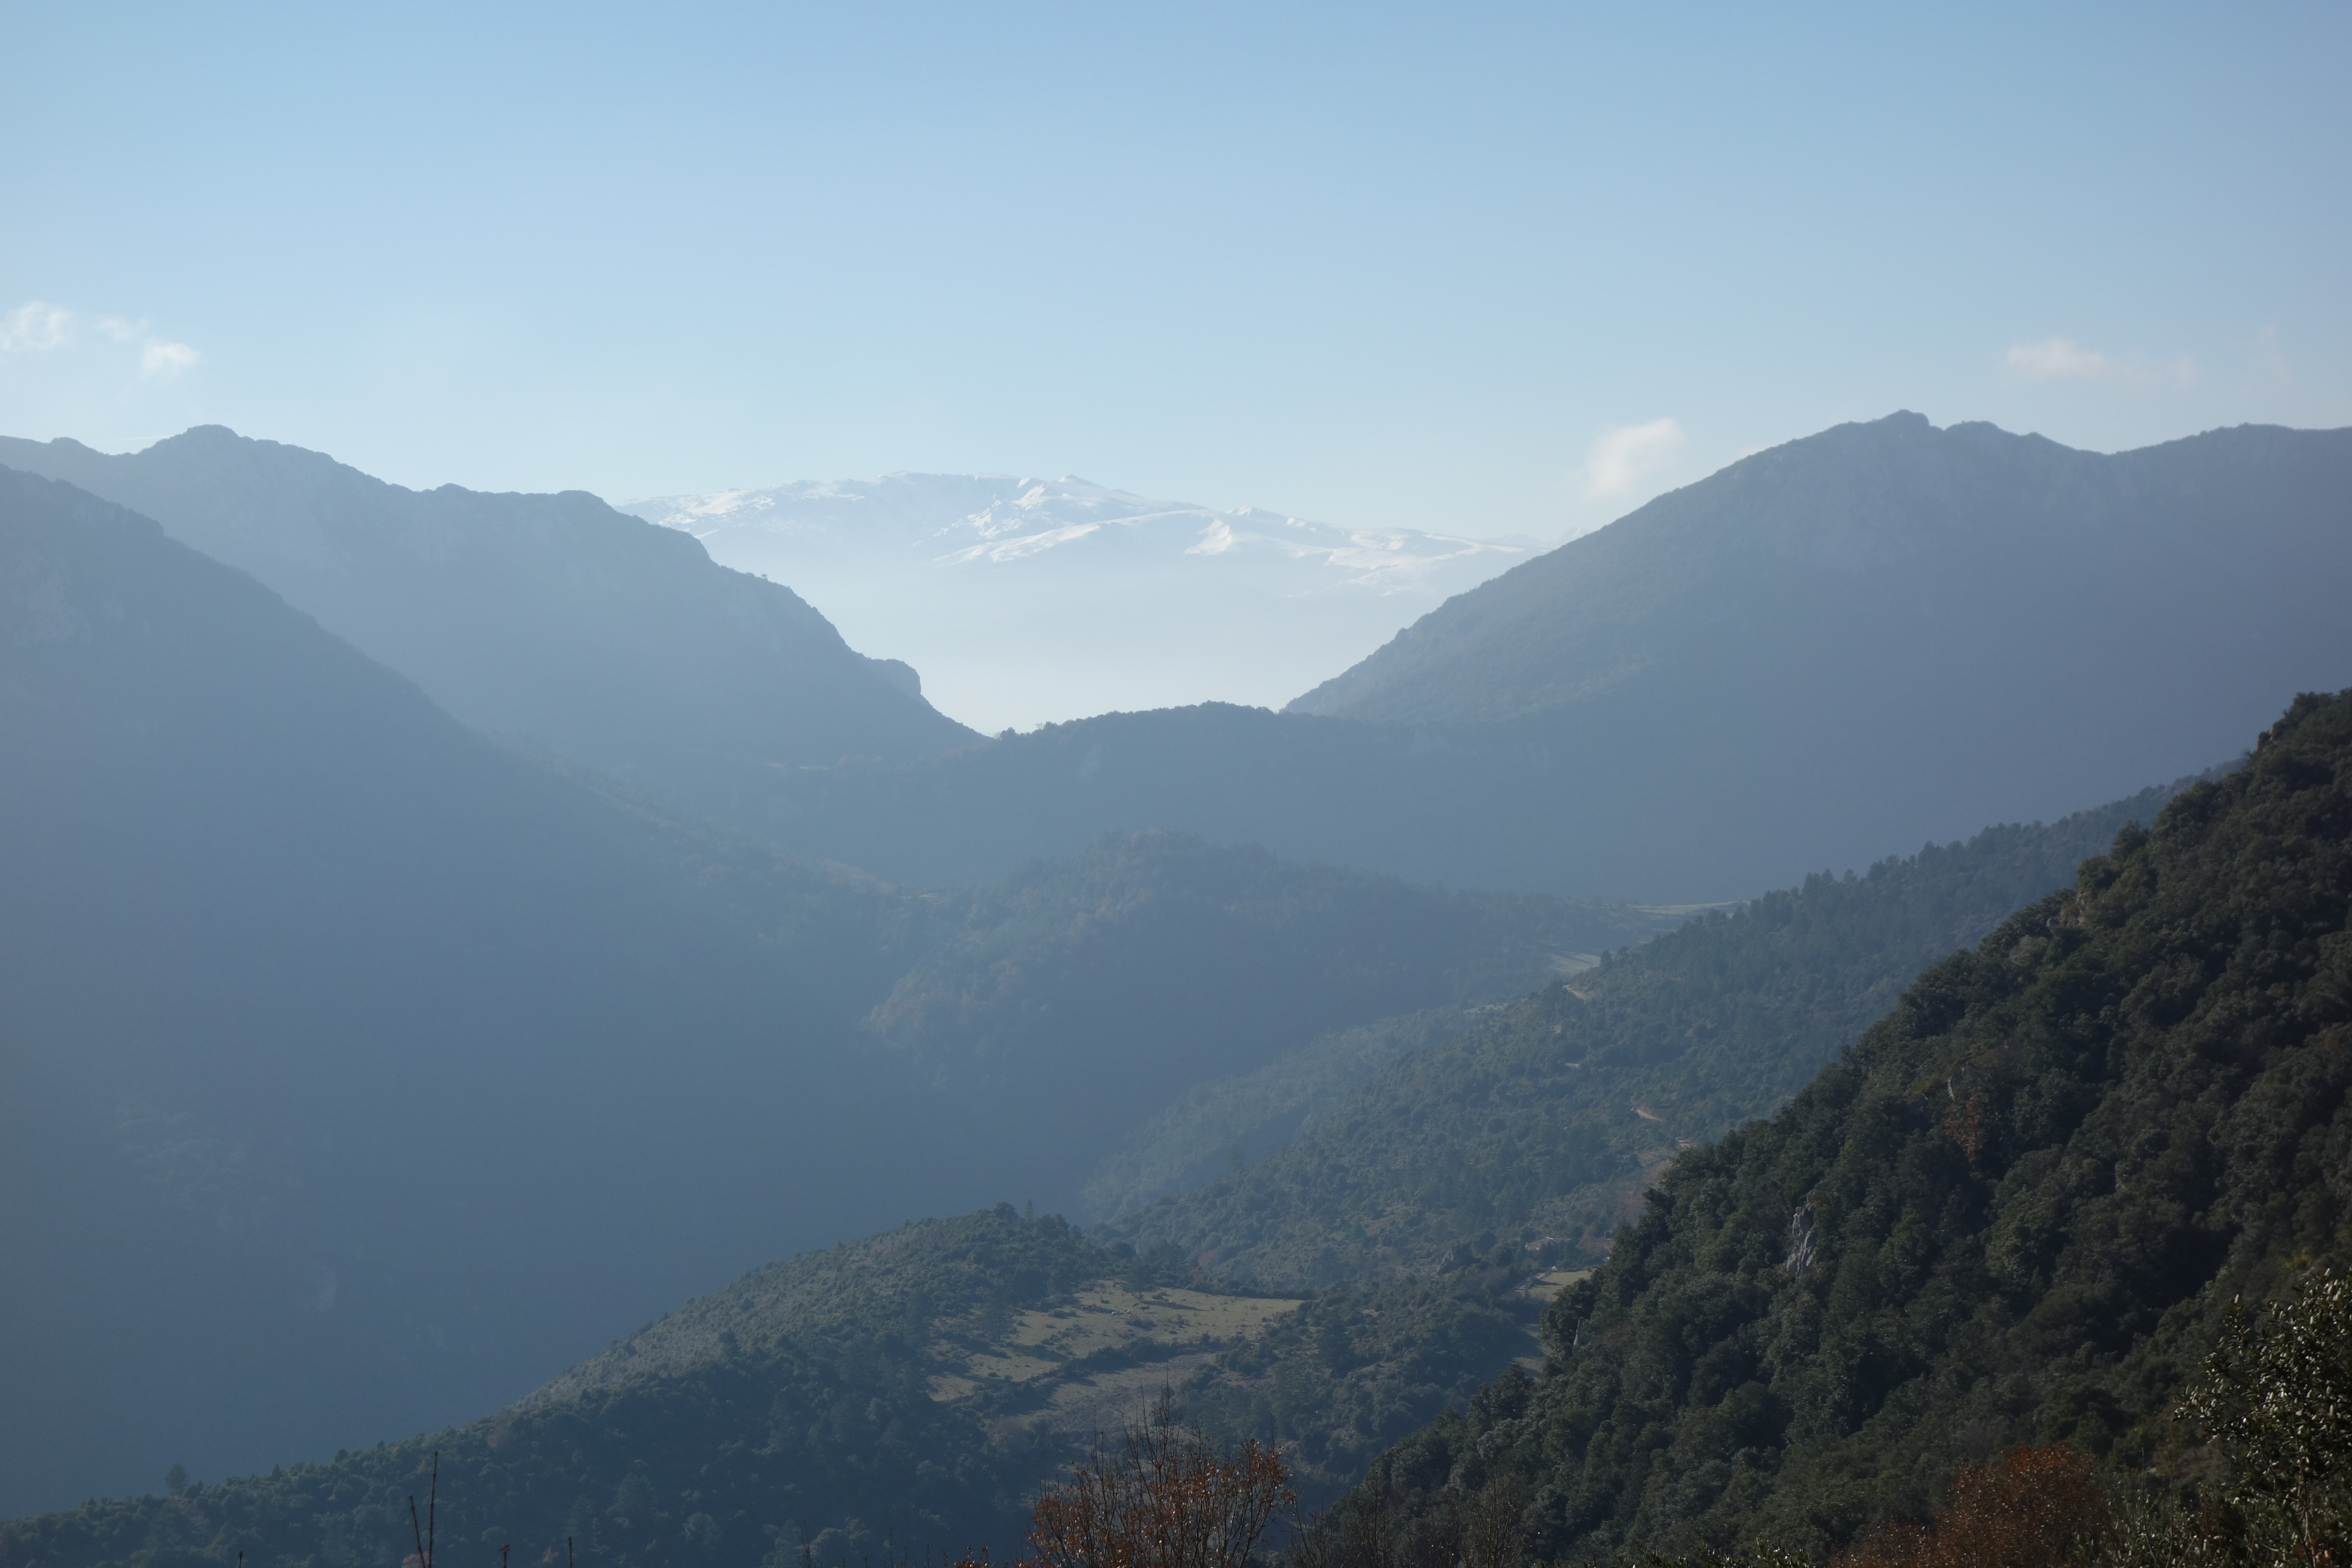
\includegraphics[width=\linewidth,height=\textheight,keepaspectratio,bb= 0 0 1126 750]{/home/mkg/Dropbox/images/DSC02788.JPG}
\captionlistentry[figure]{\url{\protect\detokenize{DSC02788.JPG}}}
\end{figure}
    
\clearpage
\onecolumn
\noindent Christmas scene, Chatham, New Jersey.
\noindent
\begin{lstlisting}

Filename: DSC03275.JPG

Date: 2013:12:25 21:20:12
Make: SONY
Model: DSC-RX100
Focal length (35mm eq): 59
Exposure: 0.03333333333333333
F stop: 3.5
ISO: 3200
Width: 5472
Height: 3648
\end{lstlisting}
\clearpage

\begin{figure}
\includegraphics[width=\linewidth,height=\textheight,keepaspectratio,bb= 0 0 1126 750]{/home/mkg/Dropbox/images/DSC03275.JPG}
\captionlistentry[figure]{\url{\protect\detokenize{DSC03275.JPG}}}
\end{figure}
    
\clearpage
\onecolumn
\noindent New York Harbor from Carroll Gardens, Brooklyn, New York.
\noindent
\begin{lstlisting}

Filename: renamed/[2016-11-05_17-39-25][DSC00875][SONY][DSC-RX100][4f803edb1d9ac20236123e7787e8f734].1.jpg

Date: 2016:11:05 17:39:25
Make: SONY
Model: DSC-RX100
Focal length (35mm eq): 28
Exposure: 0.00125
F stop: 5.6
ISO: 125
Width: 5462
Height: 3632
\end{lstlisting}
\clearpage

\begin{figure}
\includegraphics[width=\linewidth,height=\textheight,keepaspectratio,bb= 0 0 1124 747]{/home/mkg/Dropbox/images/renamed/[2016-11-05_17-39-25][DSC00875][SONY][DSC-RX100][4f803edb1d9ac20236123e7787e8f734].1.jpg}
\captionlistentry[figure]{\url{\protect\detokenize{renamed/[2016-11-05_17-39-25][DSC00875][SONY][DSC-RX100][4f803edb1d9ac20236123e7787e8f734].1.jpg}}}
\end{figure}
    
\clearpage
\onecolumn
\noindent Wall, Williamsburg, Brooklyn, New York City.
\noindent
\begin{lstlisting}

Filename: renamed/[2016-11-05_16-35-08][DSC00850][SONY][DSC-RX100][11d702afddf23ab11cc11b780ffba4de].1.jpg

Date: 2016:11:06 07:35:08
Make: SONY
Model: DSC-RX100
Focal length (35mm eq): 51
Exposure: 0.003125
F stop: 4.0
ISO: 125
Width: 5472
Height: 3648
\end{lstlisting}
\clearpage

\begin{figure}
\includegraphics[width=\linewidth,height=\textheight,keepaspectratio,bb= 0 0 1126 750]{/home/mkg/Dropbox/images/renamed/[2016-11-05_16-35-08][DSC00850][SONY][DSC-RX100][11d702afddf23ab11cc11b780ffba4de].1.jpg}
\captionlistentry[figure]{\url{\protect\detokenize{renamed/[2016-11-05_16-35-08][DSC00850][SONY][DSC-RX100][11d702afddf23ab11cc11b780ffba4de].1.jpg}}}
\end{figure}
    
\clearpage
\onecolumn
\noindent Museum of the City of New-York, New York City.
\noindent
\begin{lstlisting}

Filename: renamed/[2016-11-04_16-28-55][DSC00837][SONY][DSC-RX100][48fcaa6370377afea6e483ef14f9efcd].1.jpg

Date: 2016:11:05 07:28:55
Make: SONY
Model: DSC-RX100
Focal length (35mm eq): 28
Exposure: 0.03333333333333333
F stop: 1.8
ISO: 200
Width: 5472
Height: 3648
\end{lstlisting}
\clearpage

\begin{figure}
\includegraphics[width=\linewidth,height=\textheight,keepaspectratio,bb= 0 0 1126 750]{/home/mkg/Dropbox/images/renamed/[2016-11-04_16-28-55][DSC00837][SONY][DSC-RX100][48fcaa6370377afea6e483ef14f9efcd].1.jpg}
\captionlistentry[figure]{\url{\protect\detokenize{renamed/[2016-11-04_16-28-55][DSC00837][SONY][DSC-RX100][48fcaa6370377afea6e483ef14f9efcd].1.jpg}}}
\end{figure}
    
\clearpage
\onecolumn
\noindent Quebec City, Quebec, Canada.
\noindent
\begin{lstlisting}

Filename: renamed/[2016-10-25_17-21-56][DSC00805][SONY][DSC-RX100][8e062614d3bbed5885ffb2648f83724e].1.jpg

Date: 2016:10:26 08:21:56
Make: SONY
Model: DSC-RX100
Focal length (35mm eq): 61
Exposure: 0.01
F stop: 5.0
ISO: 125
Width: 5472
Height: 3648
\end{lstlisting}
\clearpage

\begin{figure}
\includegraphics[width=\linewidth,height=\textheight,keepaspectratio,bb= 0 0 1126 750]{/home/mkg/Dropbox/images/renamed/[2016-10-25_17-21-56][DSC00805][SONY][DSC-RX100][8e062614d3bbed5885ffb2648f83724e].1.jpg}
\captionlistentry[figure]{\url{\protect\detokenize{renamed/[2016-10-25_17-21-56][DSC00805][SONY][DSC-RX100][8e062614d3bbed5885ffb2648f83724e].1.jpg}}}
\end{figure}
    
\clearpage
\onecolumn
\noindent Garret, Greenwich Village, New York City.
\noindent
\begin{lstlisting}

Filename: renamed/[2016-09-09_19-02-13][DSC00615][SONY][DSC-RX100][017d30847041035aeaa5c80728795dc7].1.jpg

Date: 2016:09:10 09:02:13
Make: SONY
Model: DSC-RX100
Focal length (35mm eq): 72
Exposure: 0.0125
F stop: 5.0
ISO: 160
Width: 5472
Height: 3648
\end{lstlisting}
\clearpage

\begin{figure}
\includegraphics[width=\linewidth,height=\textheight,keepaspectratio,bb= 0 0 1126 750]{/home/mkg/Dropbox/images/renamed/[2016-09-09_19-02-13][DSC00615][SONY][DSC-RX100][017d30847041035aeaa5c80728795dc7].1.jpg}
\captionlistentry[figure]{\url{\protect\detokenize{renamed/[2016-09-09_19-02-13][DSC00615][SONY][DSC-RX100][017d30847041035aeaa5c80728795dc7].1.jpg}}}
\end{figure}
    
\clearpage
\onecolumn
\noindent Drain, Bovina Creamery, Bovina Center, New York.
\noindent
\begin{lstlisting}

Filename: renamed/[2016-07-22_19-15-20][DSC00365][SONY][DSC-RX100][5fa29079ce1388e440851a65ae601eb8].1.jpg

Date: 2016:07:23 09:15:20
Make: SONY
Model: DSC-RX100
Focal length (35mm eq): 95
Exposure: 0.00625
F stop: 6.3
ISO: 125
Width: 5472
Height: 3648
\end{lstlisting}
\clearpage

\begin{figure}
\includegraphics[width=\linewidth,height=\textheight,keepaspectratio,bb= 0 0 1126 750]{/home/mkg/Dropbox/images/renamed/[2016-07-22_19-15-20][DSC00365][SONY][DSC-RX100][5fa29079ce1388e440851a65ae601eb8].1.jpg}
\captionlistentry[figure]{\url{\protect\detokenize{renamed/[2016-07-22_19-15-20][DSC00365][SONY][DSC-RX100][5fa29079ce1388e440851a65ae601eb8].1.jpg}}}
\end{figure}
    
\clearpage
\onecolumn
\noindent My father's sister's husband Herb, who had been a jet engine mechanic, in his model shop at home in Florida.
\noindent
\begin{lstlisting}

Filename: renamed/[2009-03-29_16-33-11][IMG_3998_2)][Canon][Canon_PowerShot_G7][d1f87e4ff942e2fee95a04206b38b641].1.jpg

Date: 2009:03:29 16:33:11
Make: Canon
Model: Canon PowerShot G7
Exposure: 0.02
F stop: 3.2
Width: 3648
Height: 2736
\end{lstlisting}
\clearpage

\begin{figure}
\includegraphics[width=\linewidth,height=\textheight,keepaspectratio,bb= 0 0 1459 1094]{/home/mkg/Dropbox/images/renamed/[2009-03-29_16-33-11][IMG_3998_2)][Canon][Canon_PowerShot_G7][d1f87e4ff942e2fee95a04206b38b641].1.jpg}
\captionlistentry[figure]{\url{\protect\detokenize{renamed/[2009-03-29_16-33-11][IMG_3998_2)][Canon][Canon_PowerShot_G7][d1f87e4ff942e2fee95a04206b38b641].1.jpg}}}
\end{figure}
    
\clearpage
\onecolumn
\noindent In my father's sister's home, Florida.
\noindent
\begin{lstlisting}

Filename: renamed/[2009-03-29_13-58-00][IMG_3991][Canon][Canon_PowerShot_G7][0e450e9db99082f2bd8fecfaf333953f].1.jpg

Date: 2009:03:29 13:58:00
Make: Canon
Model: Canon PowerShot G7
Exposure: 0.025
F stop: 2.8
Width: 3648
Height: 2736
\end{lstlisting}
\clearpage

\begin{figure}
\includegraphics[width=\linewidth,height=\textheight,keepaspectratio,bb= 0 0 1459 1094]{/home/mkg/Dropbox/images/renamed/[2009-03-29_13-58-00][IMG_3991][Canon][Canon_PowerShot_G7][0e450e9db99082f2bd8fecfaf333953f].1.jpg}
\captionlistentry[figure]{\url{\protect\detokenize{renamed/[2009-03-29_13-58-00][IMG_3991][Canon][Canon_PowerShot_G7][0e450e9db99082f2bd8fecfaf333953f].1.jpg}}}
\end{figure}
    
\clearpage
\onecolumn
\noindent Toy display, Borough Park, Brooklyn, New York.
\noindent
\begin{lstlisting}

Filename: renamed/[2013-03-10_16-46-34][DSC01069][SONY][DSC-RX100][9efc31162858a51f6e3e6332aca8a187].1.jpg

Date: 2013:03:10 16:46:34
Make: SONY
Model: DSC-RX100
Focal length (35mm eq): 84
Exposure: 0.00125
F stop: 6.3
ISO: 125
Width: 5472
Height: 3648
\end{lstlisting}
\clearpage

\begin{figure}
\includegraphics[width=\linewidth,height=\textheight,keepaspectratio,bb= 0 0 1126 750]{/home/mkg/Dropbox/images/renamed/[2013-03-10_16-46-34][DSC01069][SONY][DSC-RX100][9efc31162858a51f6e3e6332aca8a187].1.jpg}
\captionlistentry[figure]{\url{\protect\detokenize{renamed/[2013-03-10_16-46-34][DSC01069][SONY][DSC-RX100][9efc31162858a51f6e3e6332aca8a187].1.jpg}}}
\end{figure}
    
\clearpage
\onecolumn
\noindent Collectibles shop, Greenwich Village, New York City.
\noindent
\begin{lstlisting}

Filename: renamed/[2013-05-01_19-26-15][DSC01348][SONY][DSC-RX100][56ee9f69d83e82ba490c944db6e32d55].1.jpg

Date: 2013:05:01 19:26:15
Make: SONY
Model: DSC-RX100
Focal length (35mm eq): 100
Exposure: 0.01
F stop: 4.9
ISO: 800
Width: 5472
Height: 3648
\end{lstlisting}
\clearpage

\begin{figure}
\includegraphics[width=\linewidth,height=\textheight,keepaspectratio,bb= 0 0 1126 750]{/home/mkg/Dropbox/images/renamed/[2013-05-01_19-26-15][DSC01348][SONY][DSC-RX100][56ee9f69d83e82ba490c944db6e32d55].1.jpg}
\captionlistentry[figure]{\url{\protect\detokenize{renamed/[2013-05-01_19-26-15][DSC01348][SONY][DSC-RX100][56ee9f69d83e82ba490c944db6e32d55].1.jpg}}}
\end{figure}
    
	
\end{document}

